\documentclass{article}

\usepackage{graphicx}
\usepackage{tikz}
\usepackage{tikzsymbols}
\usetikzlibrary{calc,patterns,shapes.geometric}
\pagestyle{empty}
\usepackage[margin=0pt]{geometry}
\geometry{papersize={14in,12in}}

\def\centerarc[#1](#2)(#3:#4:#5){\draw[#1] ($(#2)+({#5*cos(#3)},{#5*sin(#3)})$) arc (#3:#4:#5);}

\begin{document}
	\begin{figure}
		\centering
		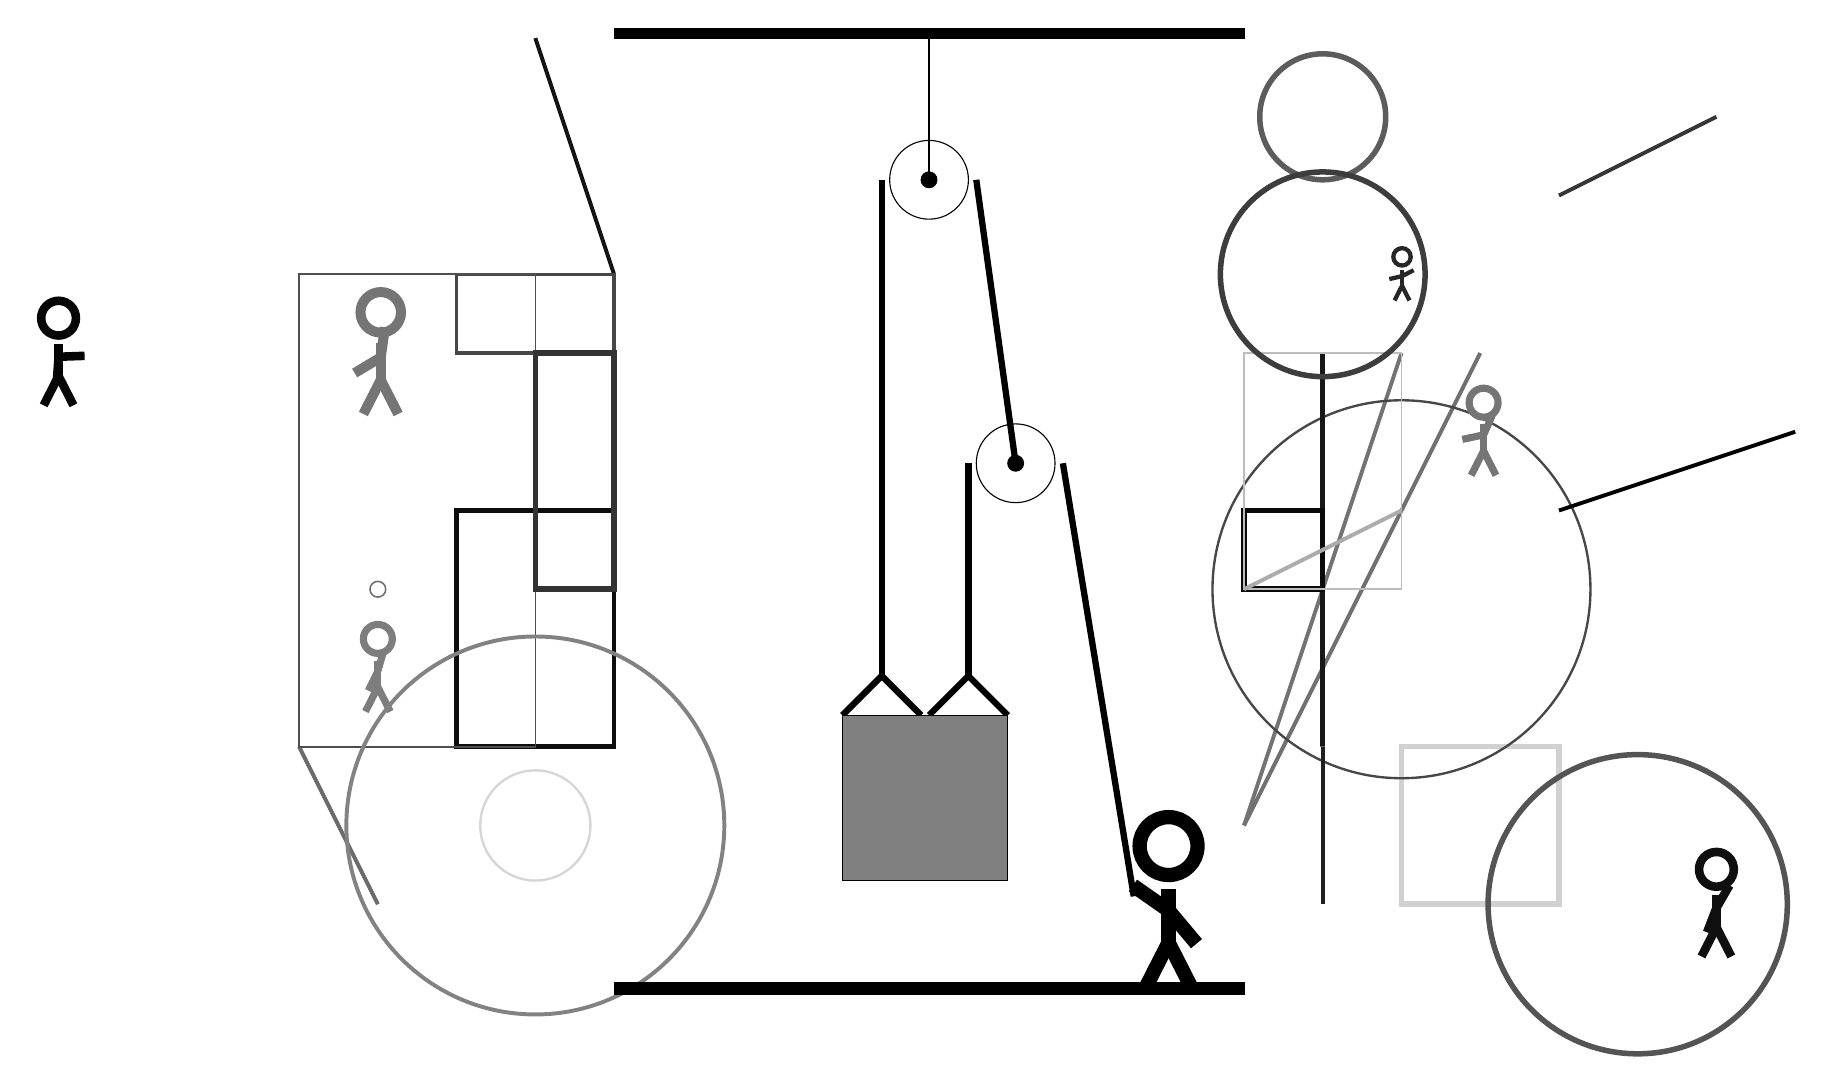
\begin{tikzpicture}
			%%%%% START %%%%%
			
			\draw[fill=black] (-2, 9) rectangle (6, 9.125);
			
			\draw (2, 7.2) circle (0.5);
			\draw[fill=black] (2, 7.2) circle (0.1);
			\draw[thick] (2, 7.2) -- (2, 9);
			
			\draw[line width=0.6mm, color=black!95] (-4, 0) rectangle (-2, 3);
			
			\draw[line width=0.7mm, color=black!18] (8, 0) rectangle (10, -2);
			\draw [line width=0.2mm, color=black!25](7, 0) circle (0.0);
			\draw[line width=0.5mm, color=black!58](-6, 0) -- (-5, -2);
			\draw[line width=0.5mm, color=black!92](-3, 9) -- (-2, 6);
			\draw[line width=0.5mm, color=black!56](6, -1) -- (9, 5);
			\draw[line width=0.5mm, color=black!55](6, -1) -- (8, 5);
			
			\draw [line width=0.3mm, color=black!72](8, 2) circle (2.4);
			\node[line width=0.2mm, color=black!94] at (12, -2) {\Strichmaxerl[6][69][60]};
			\node[line width=0.5mm, color=black!54] at (9, 4) {\Strichmaxerl[5][12][66]};
			\node[line width=0.2mm, color=black!85] at (8, 6) {\Strichmaxerl[3][13][27]};
			\draw[line width=0.4mm, color=black!72] (-4, 6) rectangle (-2, 5);
			\draw[line width=0.2mm, color=black!69] (-3, 0) rectangle (-6, 6);
			
			\node[line width=0.5mm, color=black!54] at (-5, 5) {\Strichmaxerl[7][31][82]};
			\draw [line width=0.7mm, color=black!67](11, -2) circle (1.9);
			\draw[line width=0.7mm, color=black!91] (7, 5) rectangle (7, 0);
			\draw[line width=0.7mm, color=black!96] (7, 3) rectangle (6, 2);
			\draw [line width=0.3mm, color=black!16](-3, -1) circle (0.7);
			\node[line width=0.6mm, color=black!98] at (-9, 5) {\Strichmaxerl[6][86][2]};
			\draw[line width=0.5mm, color=black!100](10, 3) -- (13, 4);
			\node[line width=0.5mm, color=black!51] at (-5, 1) {\Strichmaxerl[5][64][74]};
			\draw[line width=0.7mm, color=black!80] (-3, 5) rectangle (-2, 2);
			\draw[line width=0.5mm, color=black!79](10, 7) -- (12, 8);
			\draw [line width=0.7mm, color=black!64](7, 8) circle (0.8);
			\draw [line width=0.5mm, color=black!49](-3, -1) circle (2.4);
			
			\draw[line width=0.5mm, color=black!88](7, -2) -- (7, 0);
			
			\draw[line width=0.2mm, color=black!26] (8, 2) rectangle (6, 5);
			\draw[line width=0.5mm, color=black!33](8, 3) -- (6, 2);
			\draw [line width=0.7mm, color=black!76](7, 6) circle (1.3);
			
			\draw [line width=0.2mm, color=black!57](-5, 2) circle (0.1);
			
			\draw (3.1, 3.6) circle (0.5);
			\draw[fill=black] (3.1, 3.6) circle (0.1);
			
			\draw[line width = 0.8mm]  (0.9, 0.4) -- (1.4, 0.9) -- (1.9, 0.4);
			\draw[line width = 0.8mm]  (2.0, 0.4) -- (2.5, 0.9) -- (3.0, 0.4);
			\draw[fill=black!50] (0.9, 0.4) rectangle (3.0, -1.7);
			
			\draw[line width = 0.8mm] (1.4, 7.2) -- (1.4, 0.9);
			\centerarc[line width = 0.8mm](2, 7.2)(0:180:0.6);
			\draw[line width = 0.8mm] (2.6, 7.2) -- (3.1, 3.6);
			\draw[line width = 0.8mm] (2.5, 3.6) -- (2.5, 0.9);
			\centerarc[line width = 0.8mm](3.1, 3.6)(0:180:0.6);
			\draw[line width = 0.8mm] (3.7, 3.6) -- (4.6, -1.9);
			
			\node at (5, -2) {\Strichmaxerl[10][-35][-50]};
			
			\draw[fill=black] (-2, -3) rectangle (6, -3.15);
			
			%%%%% END %%%%%
		\end{tikzpicture}
	\end{figure}	
\end{document}